\section{Deep Learning}
Deep neural networks (DNNs) have revolutionized the field of NLP along with many others. NLP has seen three main architectures emerge over time: fully connected neural networks (FCNN), recurrent neural networks (RNNs), and Transformers.

\subsection{Fully Connected Neural Networks}
FCNNs are the simplest form of neural networks and are characterized by their feedforward structure, where the input is mapped to one or more output nodes, and with an adjustable number of hidden layers in between.
Each node is connected to every other node in the previous and following layer, via a linear transformation (i.e. a matrix multiplication) followed by a non-linear activation function (e.g. a sigmoid).
The addition of a non-linear activation function allows for the capture of non-linear relationships between the input and output, without it the transformation could be rewritten as just a single matrix multiplication.
The key advantage of DNNs is their ability to automatically learn complex representations of the input data using multiple hidden layers, allowing for the capture of high-level features that could not be easily hand-engineered.

\begin{figure}[h]
    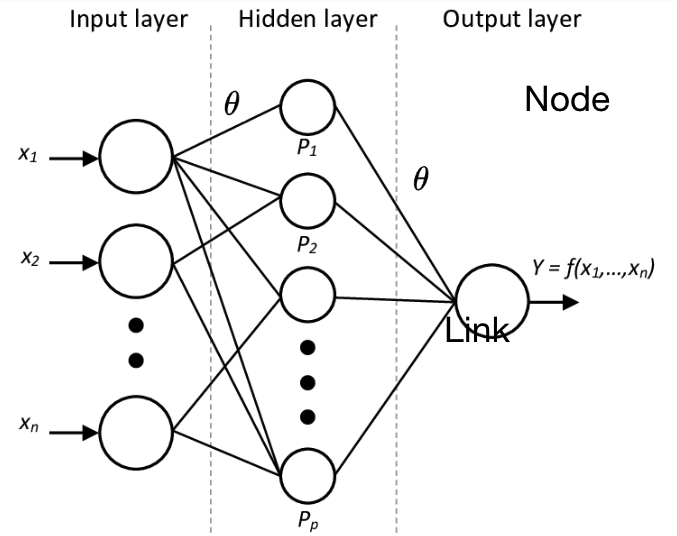
\includegraphics[width=\linewidth]{chapters/NLP/figures/model_architecture.png}
    \caption{Deep neural network architecture}
    \label{fig:model_architecture}
\end{figure}

While glossing over some details, training any type of DNN can summarized in the following steps:
\begin{itemize}
    \item Given data pairs $(x_i, y_i)$, where $x_i$ is an input sample, and $y_i$ is the desired output
    \item Determine a function $f$, such that $f(\theta, x_i) = \hat{y}_i \approx y_i$, where $\theta$ are model parameters and $f$ is the model architecture
    \item Define a loss function $L(\theta) = \sum_i L(\hat{y}_i, y_i)$ that measures how close the model's output is to the desired output
    \item Optimize $\theta$ to minimize $L(\theta)$
\end{itemize}
\begin{figure}[h]
    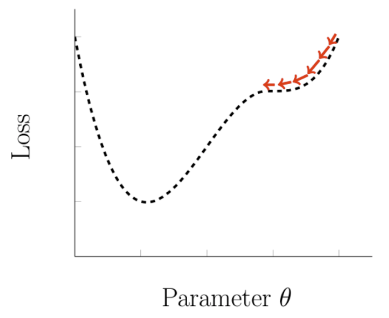
\includegraphics[width=\linewidth]{chapters/NLP/figures/loss.png}
    \caption{Minimizing the loss function}
    \label{fig:loss}
\end{figure}
Here the loss function can take on many forms, depending on the training task, we summarize some of the most common ones in Table \ref{table:losses}.
\begin{table}
    \centering
    \renewcommand{\arraystretch}{1.3}
    \begin{tabular}{|c| c| c|}
    Loss Name & Function & Use \\[0.5ex] \hline
    Mean Squared Error & $\begin{array} {lcl} \frac{1}{N} \sum_{i=1}^N|\hat{y}_i - y_i|^2\end{array}$  & regression \\ [0.5ex]
    Binary Cross Entropy & $\begin{array} {r@{}l@{}} -\frac{1}{N} \sum_{i=1}^N (y_i \cdot log(\hat{y}_i) + (1 - y_i) \cdot log(1-\hat{y}_i)) \end{array}$ & binary classification \\ [0.5ex]
    Cross Entropy & $\begin{array} {r@{}l@{}} -\frac{1}{N} \sum_{i=1}^N y_i \cdot log(\hat{y}_i) \end{array}$ & multiclass classification \\ [0.5ex]
    \end{tabular}
    \caption{Loss functions}
    \label{table:losses}
\end{table}
Training is then formulated as the task of finding the parameter configuration that minimizes the loss function.
We visualize the loss function of just a single parameter in Fig. \ref{fig:loss}.
In order to move towards the global minimum we need to update the parameters in the direction of the steepest descent, which can be calculated by taking the derivative of the loss function with respect to the parameter.
Parameters in the last layer are then updated according to the following rule until convergence
\begin{equation}
    \label{eq:optimization}
    \theta \rightarrow \theta - \alpha \frac{\partial L}{\partial \theta}
\end{equation}
where $\alpha$ is called the \textit{learning rate} and determines the step size, the partial derivative of the loss function with respect to the parameters is called the \textit{gradient}.
Consequently the algorithm is called \textit{Gradient Descent} and is the workhorse of all modern deep learning.
The algorithm trivially extends to the case of multiple parameters in the last layer.
A similar rule applies to parameters in the hidden layers.
Once the gradients of the subsequent layer have been computed we can apply the chain rule from calculus to compute the gradients of the parameters in the current layer -- this is called \textit{Backpropagation}\footnote{Backpropagation}.
% \footnote{https://en.wikipedia.org/wiki/Backpropagation}.

Simple FCNNs have several limitations in NLP.
For example, it is difficult to capture the sequential structure of text data, and they do not scale well to large vocabularies.
Remember, that in order to represent a word in a FCNN, we need to have a one-hot vector of size $|V|$.
To represent a sentence of length $n$, we need to have $n$ vectors of size $|V|$, which is a lot of parameters.

\subsection{Recurrent Neural Networks}
To overcome this, RNNs were introduced.
\begin{figure}[h]
    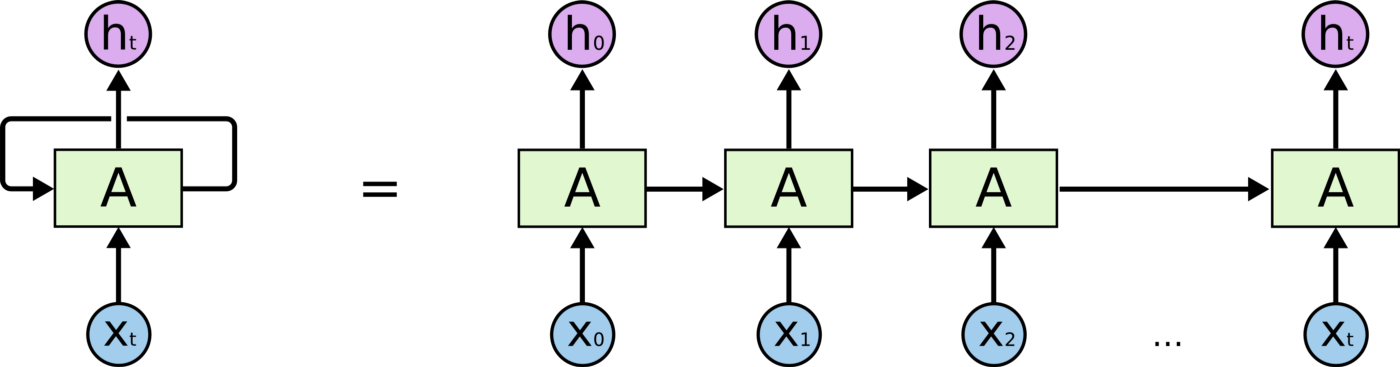
\includegraphics[width=\linewidth]{chapters/NLP/figures/rnn.png}
    \caption{Recurrent Neural Networks capture the sequential nature of text data by using loops in their structure that allow information to flow both forward and backward through the network.}
    \label{fig:rnn}
\end{figure}
RNNs are a type of neural network that have loops in their structure, allowing information to flow both forward and backward through the network (see Fig. \ref{fig:rnn}).
The idea is that we can use the output of the previous step as input to the current step, and the output of the current step as input to the next step and so on.
To encode the meaning of a sentence or paragraph, the model reads the tokens one by one, updating the representation in the hidden state, which can then be used for subsequent predictions.
This allows us to reuse a large part of the parameters, which is crucial for efficient training.
It also means that this architecture is suitable to varying length inputs, as we can stop reading the input once we reach the end of the sentence, which is in contrast to FCNNs, where we have to define the maximum length of the input in advance.
However, this comes at a cost.

For the purpose of training this architecture, you can think of unrolling the network into a sequence of layers, where each layer is a single step in the sequence.
This quickly leads to very deep neural networks, which tend to be difficult to train because the training signal has to flow through each layer.
This is related to a common problem in DL that is known as \textit{vanishing gradients}\footnote{Vanishing gradient problem}
%\footnote{\url{https://en.wikipedia.org/wiki/Vanishing_gradient_problem}}.
It occurs when the gradients used to update the network's parameters become extremely small, a consequence of the backpropagation algorithm where gradients are multiplied by the derivate of the activation function of the subsequent layer.
In the case of a $sigmoid$ its derivative is smaller than one, so that this factor decays exponentially in the number of layers.
This means that the maximum sequence length that can be learned is strongly limited.
There are some workarounds, such as using different activation functions\footnote{$tanh$, $ReLU$} or gating mechanisms\footnote{Long Short-Term Memory (LSTM)}\footnote{Gated Recurrent Units (GRU)} to allow the information to propagate more freely through the network.
But even then, the maximum achievable sequence length is limited to about 100 tokens before the network "forgets" what happens at the beginning.

Lastly, RNNs are inherently sequential because the output of a step depends on the output of the previous step, and vice versa during backpropagation.
We can not parallelize this process making parameter updates, and therefore scaling to large datasets, as well as inference very slow.

\subsection{Attention}
Attention is a mechanism that allows the model to focus on different parts of the input sequence in parallel.

\subsection{Transformers}
Transformers are a type of neural network that is based on self-attention, which allows the network to attend to different parts of the input sequence in parallel.
This allows transformers to effectively capture long-term dependencies in sequential data, without the limitations of the vanishing gradient problem.

Transformers have proven to be highly effective in NLP, and have become the state-of-the-art architecture for many tasks, including machine translation, text classification, and question answering.
This is largely due to the ability of transformers to effectively capture the relationships between different parts of the input sequence, which is critical for NLP tasks where understanding the context and relationships between words is important.

There have been significant advancements in ML due to a variety of factors, such as the availability of larger and larger datasets, as well as ever increasing computational power at lower and lower prices, better software tools, libraries and model architectures.
Especially the advent of deep learning (DL), fueled by the emergence of GPUs from about 2012, enabled scaling to many orders of magnitude larger datasets and models.
The common wisdom before DL was that as the number of parameters in a model increases beyond a certain threshold, it tends to overfit the training data, leading to poor generalization when deployed in the real world.
Deep Learning based models empirically do not seem to exhibit this behavior, and instead tend gain performance as they get bigger, albeit more slowly.

Until recently, building strong NLP systems required deep understanding of language and its structure, as well as large amounts of data, even when relying on pre-trained word embeddings - the resulting systems were often still brittle.

% In recent years some surprisingly powerful architectures and pre-training regimes have emerged that build on the concepts we have discussed here, most notably under the name of \textit{Transformers\footnote{BERT, GPT}}, that address the last bullet point of our representation's shortcomings.

The details of the inner workings are beyond the scope of this tutorial, for now it suffices to know that they are able to learn robust sentence embeddings with a fine grained understanding of syntactic structure, semantics, and general knowledge of the world.
In fact, they can be considered near the level of a human that just knows the English language (or other languages), along with a broad array of factual knowledge about the world (think Wikipedia).
Just like a human, they can be taught specialty knowledge that is relevant to a given task, in ML we would say we \textit{finetune} them.
% Where these models to date generally fall short is in terms of logical inference.
This paradigm shift has led to a step function improvement in terms of performance and sample efficiency in a wide variety of NLP tasks where Transformers are the defacto state of the art.

In the following sections, we will discuss a broad set of problem statements Transformers are suitable for, along with a set of techniques a practitioner can employ to arrive at robust solutions, even with limited data.

\subsection{Pre-training}
Modern DL-based systems, such as the aforementioned Transformer architectures, are pre-trained on gigantic datasets\footnote{BooksCorpus (800M words, Wikipedia 2,500M words)}\cite{bertpaper} and can be downloaded for free\footnote{Huggingface}.
Starting with a model pre-trained on a broad set of topics significantly reduces the amount of task specific training data required to achieve a given performance.
Furthermore, it may be helpful to start with a model that is pre-trained on more domain-specific datasets such as \texttt{BioBERT\cite{DBLP:journals/corr/abs-1901-08746}} or \texttt{Bio\textunderscore ClinicalBERT\cite{clinicalbert}}, or pre-train your model from scratch.

\subsection{Practical Considerations}
In contemporary architectures there are millions to hundreds of billions of parameters, and updating them efficiently is crucial.

To optimize the parameters as outlined in Eq. \ref{eq:optimization} we need to evaluate the gradient of the loss function given the data $(x_i, y_i)$.
To compute the optimial update step we need to sum over all samples in the dataset, compute and store all the gradients, update the parameters once, and repeat the process until convergence.
This, however is not practical, given the size of typical datasets and the number of model parameters -- each step would be very computationally expensive and the training slow.

On the other end of the spectrum we could use only a single sample to compute approximations of the optimal gradients, and they will take us close to the global minimum.
This method is called \textit{stochastic gradient descent} and generally works well, but it comes with some tradeoffs:
\begin{itemize}
    \item Loading single samples from the dataset is slow, due to CPU, RAM and bus overhead when copying data to VRAM
    \item There is overhead in the GPU related to scheduling of compute operations
    \item The gradients are much more noisy than the optimal ones, and the model will learn more slowly (see Fig. \ref{fig:mini-batch})
\end{itemize}
There is a happy middle ground called \textit{mini-batch gradient descent} which is a combination of stochastic gradient descent with mini-batches.
Using mini-batches allows for a more accurate estimate of the gradient, and reduces the overhead per sample, as we can take advantage of hardware accelerated vectorized compute operations in CPUs and GPUs.
In practice, we will choose a batch size that is much smaller than the number of samples in the dataset, and as big as possible without running out of VRAM, where the latter condition is typically the more relevant constraint.

\begin{figure}[h]
    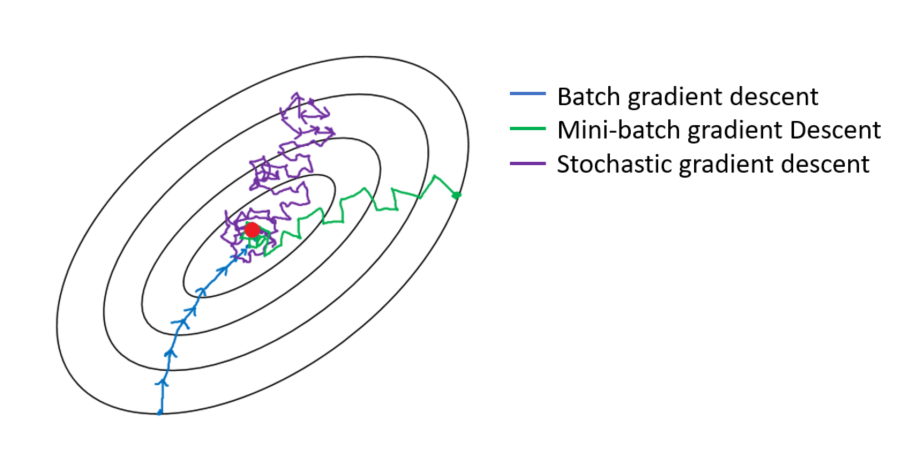
\includegraphics[width=\linewidth]{chapters/NLP/figures/mini-batch.png}
    \caption{Batch vs mini-batch vs stochastic gradient descent}
    \label{fig:mini-batch}
\end{figure}
